\documentclass[tikz, border=10pt]{standalone}
\usepackage{pgfplots}
\pgfplotsset{compat=1.18}

\begin{document}
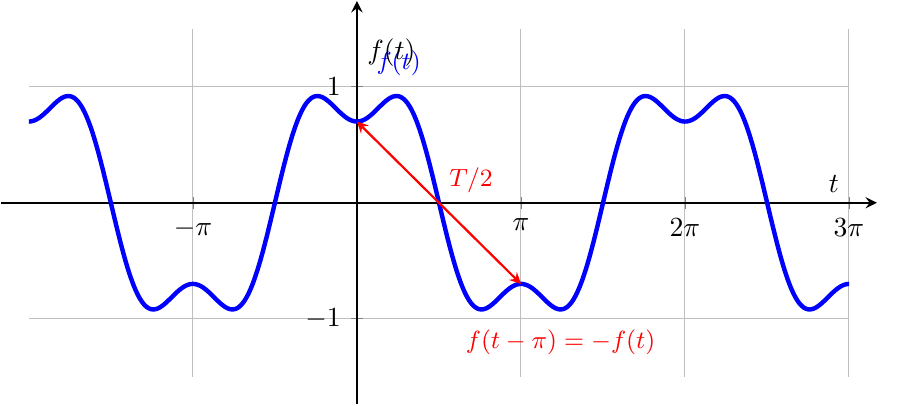
\begin{tikzpicture}
    \begin{axis}[
        width=12cm, height=6cm,
        axis lines=middle,
        xlabel={$t$}, ylabel={$f(t)$},
        ymin=-1.5, ymax=1.5,
        xmin=-2*pi, xmax=3*pi,
        xtick={-3.14, 0, 3.14, 6.28, 9.42},
        xticklabels={$-\pi$, 0, $\pi$, $2\pi$, $3\pi$},
        grid=both,
        samples=400,
        domain=-2*pi:3*pi,
        thick,
        axis line style={shorten >=-10pt, shorten <=-10pt}
    ]
        % Even + HWS: f(t) = cos(t) - 0.3*cos(3t)
        % Period T = 2pi, T/2 = pi
        % f(t-pi) = cos(x-pi) - 0.3*cos(3(x-pi)) = -cos(x) + 0.3*cos(3x) = -f(x)
        \addplot[blue, ultra thick] {cos(deg(x)) - 0.3*cos(deg(3*x))};
        
        \node[blue] at (axis cs:0.8, 1.2) {\small $f(t)$};
        \node[red] at (axis cs:3.9, -1.2) {\small $f(t-\pi) = -f(t)$};
        
        % Annotations for HWS
        \draw[<->, >=stealth, red, thick] (axis cs:0, 0.7) -- (axis cs:3.14, -0.7) node[midway, above right] {\small $T/2$};
    \end{axis}
\end{tikzpicture}
\end{document}
